\documentclass[Report.tex]{subfiles}
\externaldocument[I-]{chapter_1_introduction.tex}
\externaldocument[M-]{chapter_2_method.tex}
\externaldocument[D-]{chapter_3_discardMethod.tex}
\externaldocument[C-]{chapter_5_conclusion.tex}
\externaldocument[RE-]{chapter_6_recognition.tex}

\begin{document}
\chapter{Result - Discussion}
\label{chap:Result - Discussion}
\section{Result: Text Segmentation}
We tried 3 Approaches, Morphological, Stroke Width Transform and OpenCv Scene text detection. We end up with the simple solution Morphological approach. It gave good result, but have a lot of limitations. Only work on black text on white paper, image with little noise and only want text in the image. It work in our project. 

\section{Result: Preprocessing}
\begin{figure}[ht]
  \centering
  \begin{subfigure}[t]{4cm}
    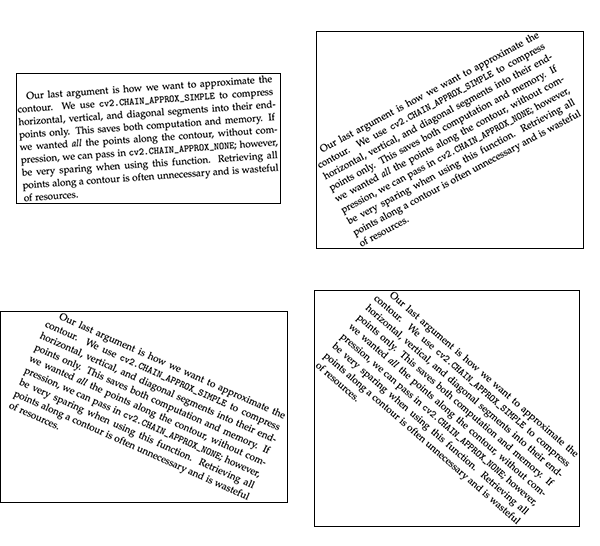
\includegraphics[width=3cm]{res/segment_text1.png}
    \caption{Example 1, Good result on just text}
  \end{subfigure}
  \hspace{5mm}%
  \begin{subfigure}[t]{4cm}
    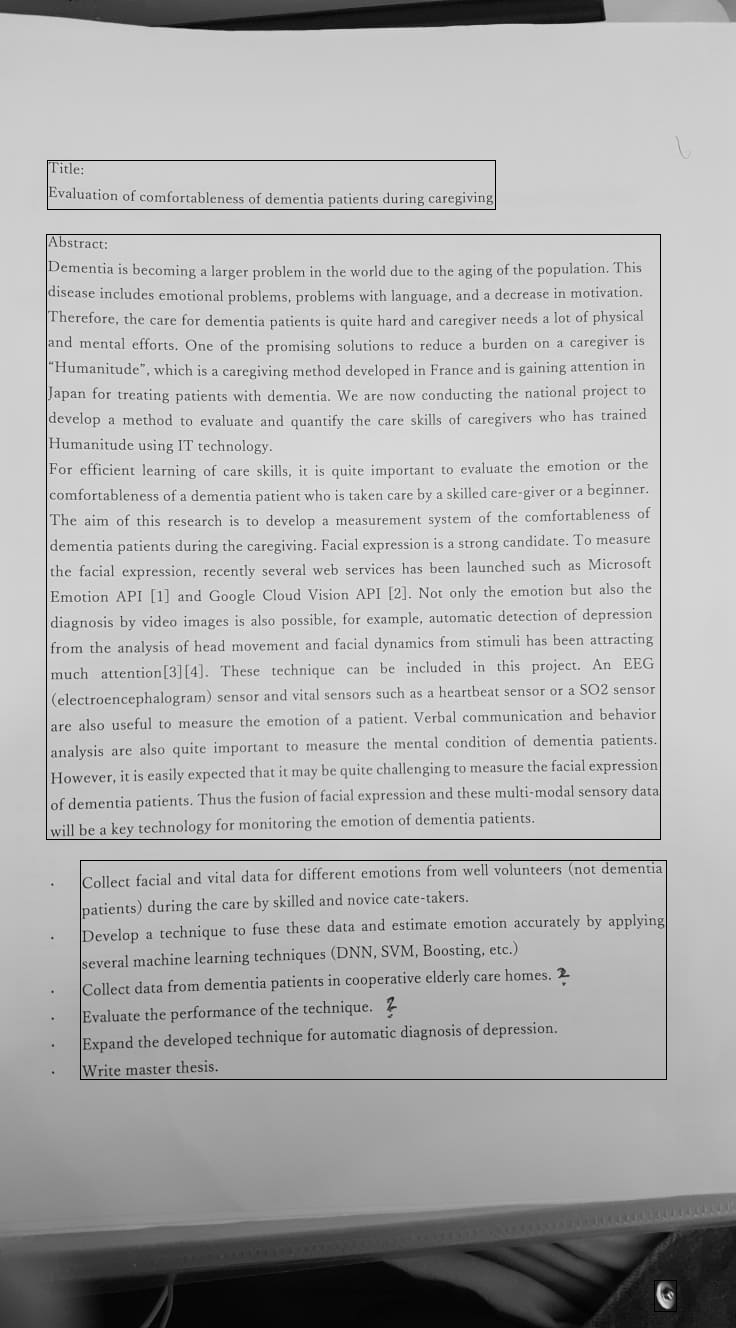
\includegraphics[width=3cm]{res/segment_text2.png}
    \caption{Example 2, Good result on paper}
  \end{subfigure}
  \hspace{5mm}%
  \begin{subfigure}[t]{4cm}
    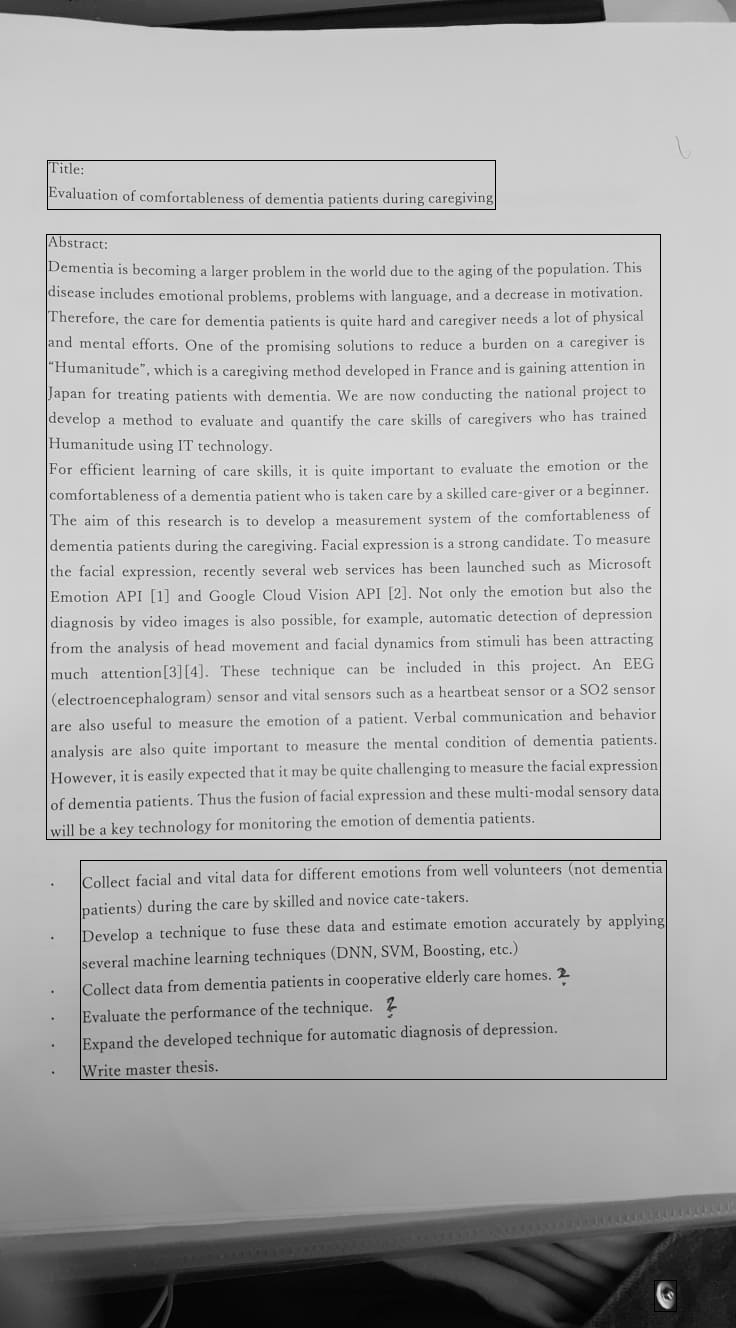
\includegraphics[width=3cm]{res/segment_text3.png}
    \caption{text}
  \end{subfigure}
  \caption{Example 3, Part of the text was not included}
  \label{fig:Text_detection_approaches}
\end{figure}

\subsection{Rotation}
\todo[inline]{
  We tried this approach, however we would end up with several lines on a text
  segment, both along the vertical and horizontal direction of the text. However
  the lines were not restricted to just these directions, we sometimes got lines
  where there where no apperant reason for it to be. Because of these
  uncertainties we tried another approach, minAreaRect method from OpenCV, see
  bellow.
}
\subsection{Line segmentation}



\todo[inline]{include results from line segmentation}

\begin{figure}[H]
  \centering
  
\includegraphics[height=4cm]{res/4angle_rot.png}
  \caption{cv.minAreaRect cannot differentiate between 0\textdegree and 180\textdegree, and 90\textdegree and 270\textdegree}
  \label{fig:4angle_rot}
\end{figure}



\subsection{Character segmentation}

\section{Result: Classification}
\section{Result: Datasets}


\end{document}
